\documentclass[tikz]{standalone}
\usepackage{tikz}
\usetikzlibrary{arrows.meta,positioning,fit,shapes.multipart}
\begin{document}
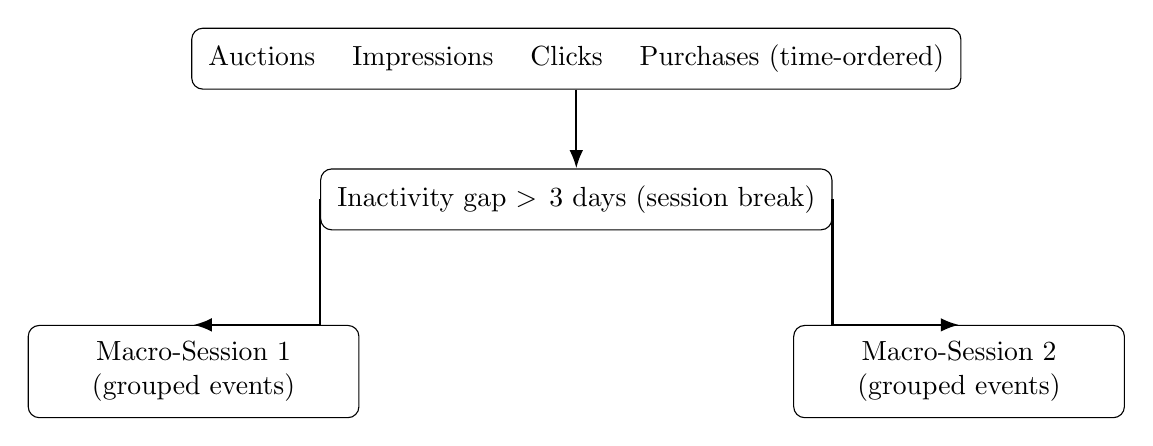
\begin{tikzpicture}[
  node distance=10mm,
  box/.style={draw, rounded corners, align=center, inner sep=6pt},
  arr/.style={-Latex, thick}
]

% Timeline of events
\node[box, minimum width=9.5cm] (events) {Auctions \quad Impressions \quad Clicks \quad Purchases (time-ordered)};

% Gap indicator
\node[box, below=of events, minimum width=5.5cm] (gap) {Inactivity gap $>\,3$ days (session break)};

% Macro-sessions
\node[box, below left=12mm and -5mm of gap, minimum width=4.2cm] (ms1) {Macro-Session 1\\(grouped events)};
\node[box, below right=12mm and -5mm of gap, minimum width=4.2cm] (ms2) {Macro-Session 2\\(grouped events)};

% Arrows
\draw[arr] (events) -- (gap);
\draw[arr] (gap.west) |- (ms1.north);
\draw[arr] (gap.east) |- (ms2.north);

% Caption-like label (optional minimal)
% \node[below=8mm of ms1, align=center] {Macro-session construction from raw event streams};

\end{tikzpicture}
\end{document}

